%%%%%%%%%%%%%%%%%%%%%%%%%%%%%%%%%%%%%%%%%%%%%%%%%%%%%%%%%%%%%%%%%%%%%%%%%%%%%%%%
% Template for USENIX papers.
%
% History:
%
% - TEMPLATE for Usenix papers, specifically to meet requirements of
%   USENIX '05. originally a template for producing IEEE-format
%   articles using LaTeX. written by Matthew Ward, CS Department,
%   Worcester Polytechnic Institute. adapted by David Beazley for his
%   excellent SWIG paper in Proceedings, Tcl 96. turned into a
%   smartass generic template by De Clarke, with thanks to both the
%   above pioneers. Use at your own risk. Complaints to /dev/null.
%   Make it two column with no page numbering, default is 10 point.
%
% - Munged by Fred Douglis <douglis@research.att.com> 10/97 to
%   separate the .sty file from the LaTeX source template, so that
%   people can more easily include the .sty file into an existing
%   document. Also changed to more closely follow the style guidelines
%   as represented by the Word sample file.
%
% - Note that since 2010, USENIX does not require endnotes. If you
%   want foot of page notes, don't include the endnotes package in the
%   usepackage command, below.
% - This version uses the latex2e styles, not the very ancient 2.09
%   stuff.
%
% - Updated July 2018: Text block size changed from 6.5" to 7"
%
% - Updated Dec 2018 for ATC'19:
%
%   * Revised text to pass HotCRP's auto-formatting check, with
%     hotcrp.settings.submission_form.body_font_size=10pt, and
%     hotcrp.settings.submission_form.line_height=12pt
%
%   * Switched from \endnote-s to \footnote-s to match Usenix's policy.
%
%   * \section* => \begin{abstract} ... \end{abstract}
%
%   * Make template self-contained in terms of bibtex entires, to allow
%     this file to be compiled. (And changing refs style to 'plain'.)
%
%   * Make template self-contained in terms of figures, to
%     allow this file to be compiled. 
%
%   * Added packages for hyperref, embedding fonts, and improving
%     appearance.
%   
%   * Removed outdated text.
%
%%%%%%%%%%%%%%%%%%%%%%%%%%%%%%%%%%%%%%%%%%%%%%%%%%%%%%%%%%%%%%%%%%%%%%%%%%%%%%%%

\documentclass[letterpaper,twocolumn,10pt]{article}
\usepackage{usenix-2020-09}

% to be able to draw some self-contained figs
\usepackage{tikz}
\usepackage{amsmath}

% inlined bib file
\usepackage{filecontents}

%-------------------------------------------------------------------------------
\begin{filecontents}{\jobname.bib}
%-------------------------------------------------------------------------------
@Book{arpachiDusseau18:osbook,
  author =       {Arpaci-Dusseau, Remzi H. and Arpaci-Dusseau Andrea C.},
  title =        {Operating Systems: Three Easy Pieces},
  publisher =    {Arpaci-Dusseau Books, LLC},
  year =         2015,
  edition =      {1.00},
  note =         {\url{http://pages.cs.wisc.edu/~remzi/OSTEP/}}
}
@InProceedings{waldspurger02,
  author =       {Waldspurger, Carl A.},
  title =        {Memory resource management in {VMware ESX} server},
  booktitle =    {USENIX Symposium on Operating System Design and
                  Implementation (OSDI)},
  year =         2002,
  pages =        {181--194},
  note =         {\url{https://www.usenix.org/legacy/event/osdi02/tech/waldspurger/waldspurger.pdf}}}
\end{filecontents}

%-------------------------------------------------------------------------------
\begin{document}
%-------------------------------------------------------------------------------

%don't want date printed
\date{}

% make title bold and 14 pt font (Latex default is non-bold, 16 pt)
\title{\Large \bf Paper Review}

%for single author (just remove % characters)
\author{
{\rm Tony\ Wang}\\
Technical University Munich
% copy the following lines to add more authors
% \and
% {\rm Name}\\
%Name Institution
} % end author

\maketitle

%-------------------------------------------------------------------------------
% \begin{abstract}
% %-------------------------------------------------------------------------------
% Your abstract text goes here. Just a few facts. Whet our appetites.
% Not more than 200 words, if possible, and preferably closer to 150.
% \end{abstract}


%-------------------------------------------------------------------------------
\section{Introduction}
%-------------------------------------------------------------------------------

Tianqi Chen, lead author of the paper holds a BS and MS from the Shanghai Jiao Tong
Universit, a PhD from the University of Washington and is currently an Assistant 
Professor at Carnegie Mellon University. At the time the article was published in 2018, 
Chen was still a PhD student at the University of Washington.

Deep learning computation requirements are increasing each year; therefore, it is imperative
to fetch every bit of performance, and optimize everywhere. Thus, new hardware need to get published to 
the market, which also creates a problem. Many of these novel hardware have different architectures. 
But current deep learning frameworks are only optimized on server-class GPUs and not for these specialized hardware,
since they are based on operator libraries. which are hand-written optimizations by software engineers. 
They delegate target-specific optimizations to highly engineered and vendor-specific operator libraries, which is 
requires experience and can cost a lot of development time. Therefore deep learning frameworks perform worse on 
many specialized hardware, for they are not optimized for them. If you want to deploy your model on a new hardware 
that your framework does not support, you might end up with bad performance.
To target this problem, Chen et al. proposed a novel end-to-end compiler called TVM (Tensor Virtual Machine), which 
can address a wide range of different hardware back-ends.

%-------------------------------------------------------------------------------
\section{Summary}
%-------------------------------------------------------------------------------

Chen et al. use in TVM an idea that dates way back to 1997 - that is optimizing the code with machine-learning.
Since then, there has been many attempts at using machine-learning (ML) for compilers.
The work of Chen et al. uses this approach to solve two fundamental problems in deep learning in one fell swoop.
It can not only target a wide range of hardware back-ends, it also generates optimized code for each of the hardware.
This process takes place in many stages, which are explained in a well-structured manner throughout the paper.
TVM takes a model from different frameworks (e.g. TensorFlow or PyTorch) and converts it into a computation graph 
for high-level graph optimizations, such as operator fusion and data layout transformation and creates an optimized graph.
Then for each operator in the graph, the operator-levle optimization module, the heart of the compiler, generates the target specific 
optimized code. In this module the schedule and execution details will be determined for the specific hardware-backend by the ML-based cost model.
The resulting code can then be deployed on different modules, like LLVM IR, CUDA, or OpenCL. TVM also implements RPC-based remote function call support,
which is crucial for embedded devices. At last the authors evaluate their new system on a server-class GPU, embedded GPU and CPU, and a custom-made FPGA-accelerator
with real world workloads, yielding promising results, by surpassing the state-of-the-art rivals in every benchmark.
%-------------------------------------------------------------------------------
\section{Review}
%-------------------------------------------------------------------------------

Deep learning frameworks depend on creating computation graphs, thus prominent deep learning frameworks such as PyTorch and 
TensorFlow make use of graph-level optimizations as well. In this area other deep learning frameworks are very similar to TVM.
For instance, TensorFLow uses Grapper as graph optimization system, using the same graph optimizations such as Constant folding optimizer, or Layout optimizer.
Chen et al. respond to this by emphasising that, in contrary to other deep learning frameworks, TVM does not rely on hand-built kernel libraries and
can therefore target a much wider area of hardware, since it is not feasible to handshape the hand-written libraries for every hardware.
Chan et al. then go into detail how operator fusion and data layout transformation work. However, I would have loved 
to see a more in-depth comparison between these graph-level optimizations between these frameworks. Since they all share similar tasks, and 
therefore implement similar operations, it would be interesting to see if the numbers of possible operations match with each other, or whether 
some graph-level optimizing operations perform better than other frameworks and vice versa.
%---------------------------
\begin{figure}
\begin{center}
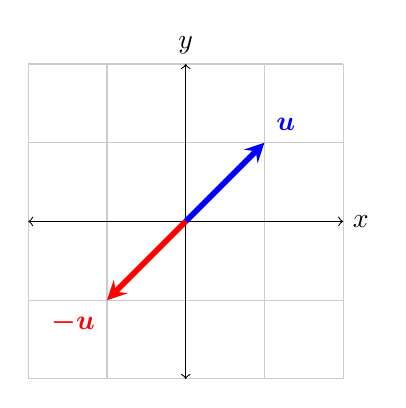
\begin{tikzpicture}
  \draw[thin,gray!40] (-2,-2) grid (2,2);
  \draw[<->] (-2,0)--(2,0) node[right]{$x$};
  \draw[<->] (0,-2)--(0,2) node[above]{$y$};
  \draw[line width=2pt,blue,-stealth](0,0)--(1,1)
        node[anchor=south west]{$\boldsymbol{u}$};
  \draw[line width=2pt,red,-stealth](0,0)--(-1,-1)
        node[anchor=north east]{$\boldsymbol{-u}$};
\end{tikzpicture}
\end{center}
\caption{\label{fig:vectors} Text size inside figure should be as big as
  caption's text. Text size inside figure should be as big as
  caption's text. Text size inside figure should be as big as
  caption's text. Text size inside figure should be as big as
  caption's text. Text size inside figure should be as big as
  caption's text. }
\end{figure}
%% %---------------------------


Here's a typical reference to a floating figure:
Figure~\ref{fig:vectors}. Floats should usually be placed where latex
wants then. Figure\ref{fig:vectors} is centered, and has a caption
that instructs you to make sure that the size of the text within the
figures that you use is as big as (or bigger than) the size of the
text in the caption of the figures. Please do. Really.

In our case, we've explicitly drawn the figure inlined in latex, to
allow this tex file to cleanly compile. But usually, your figures will
reside in some file.pdf, and you'd include them in your document
with, say, \textbackslash{}includegraphics.

Lists are sometimes quite handy. If you want to itemize things, feel
free:

\begin{description}
  
\item[fread] a function that reads from a \texttt{stream} into the
  array \texttt{ptr} at most \texttt{nobj} objects of size
  \texttt{size}, returning returns the number of objects read.

\item[Fred] a person's name, e.g., there once was a dude named Fred
  who separated usenix.sty from this file to allow for easy
  inclusion.
\end{description}

\noindent
The noindent at the start of this paragraph in its tex version makes
it clear that it's a continuation of the preceding paragraph, as
opposed to a new paragraph in its own right.


\subsection{LaTeX-ing Your TeX File}
%-----------------------------------

People often use \texttt{pdflatex} these days for creating pdf-s from
tex files via the shell. And \texttt{bibtex}, of course. Works for us.

%-------------------------------------------------------------------------------
\section*{Acknowledgments}
%-------------------------------------------------------------------------------

The USENIX latex style is old and very tired, which is why
there's no \textbackslash{}acks command for you to use when
acknowledging. Sorry.

%-------------------------------------------------------------------------------
\section*{Availability}
%-------------------------------------------------------------------------------

USENIX program committees give extra points to submissions that are
backed by artifacts that are publicly available. If you made your code
or data available, it's worth mentioning this fact in a dedicated
section.

%-------------------------------------------------------------------------------
\bibliographystyle{plain}
\bibliography{\jobname}

%%%%%%%%%%%%%%%%%%%%%%%%%%%%%%%%%%%%%%%%%%%%%%%%%%%%%%%%%%%%%%%%%%%%%%%%%%%%%%%%
\end{document}
%%%%%%%%%%%%%%%%%%%%%%%%%%%%%%%%%%%%%%%%%%%%%%%%%%%%%%%%%%%%%%%%%%%%%%%%%%%%%%%%

%%  LocalWords:  endnotes includegraphics fread ptr nobj noindent
%%  LocalWords:  pdflatex acks
